\documentclass[aspectratio=169]{beamer}
\usetheme{Madrid}
\usecolortheme{default}

\usepackage{graphicx}
\usepackage{amsmath}
\usepackage{amsfonts}
\usepackage{xcolor}
\usepackage{tikz}
\usepackage{pgfplots}

\definecolor{recon2color}{rgb}{0.8,0.2,0.1}
\definecolor{recon3color}{rgb}{0.1,0.5,0.2}

\pgfplotsset{compat=1.17}
\usetikzlibrary{patterns,arrows.meta}

\title{PCA on Functions}
\subtitle{Approximating and summarizing functions using principal components}
\author{CSE255 - Scalable Data Analysis}
\date{\today}

\begin{document}

\begin{frame}
  \titlepage
\end{frame}

% --- Link to functions as vectors ---
\begin{frame}{Functions as vectors (recap)}
  \small
  From \texttt{Functions\_as\_vectors}: a function $f$ on $[0, 2\pi]$ is a vector (samples on a grid).
  \begin{itemize}
    \item Inner product: $\langle f, g \rangle = \sum_i f(x_i)\, g(x_i)\, \Delta x$
    \item Orthonormal basis $\{u_1, u_2, \ldots\}$: reconstruction $f = \sum_i c_i u_i$ with $c_i = \langle f, u_i \rangle$.
  \end{itemize}
  \vspace{0.2cm}
  \textbf{PCA} finds a data-driven orthonormal basis (principal components) that captures maximum variance.
\end{frame}

% --- Data = collection of functions ---
\begin{frame}{Data: a collection of functions}
  \small
  \textbf{Data matrix} $\mathbf{X} \in \mathbb{R}^{n \times d}$:
  \begin{itemize}
    \item $n$ = number of functions (e.g., different signals or time series)
    \item $d$ = number of grid points (e.g., on $[0, 2\pi]$)
    \item Row $i$ = $i$-th function discretized: $[f_i(x_1), \ldots, f_i(x_d)]$
  \end{itemize}
  \vspace{0.2cm}
  Center the data: subtract the \textbf{mean function} $\boldsymbol{\mu}(x)$ (row-wise mean of $\mathbf{X}$).\\
  PCA is applied to the \textbf{centered} matrix.
\end{frame}

% --- Mean and principal component functions ---
\begin{frame}{Mean and principal component functions}
  \small
  \begin{itemize}
    \item \textbf{Mean function:} $\mu(x) = \frac{1}{n}\sum_{i=1}^n f_i(x)$ (average across samples).
    \item \textbf{Covariance} (in function space) leads to eigenfunctions.
    \item \textbf{Principal component functions} $u_1(x), u_2(x), \ldots$: orthonormal, ordered by explained variance ($\lambda_1 \geq \lambda_2 \geq \cdots$).
  \end{itemize}
  \vspace{0.2cm}
  Coefficients for a (centered) function $f - \mu$: $c_j = \langle f - \mu, u_j \rangle$.
\end{frame}

% --- Reconstruction with top K PCs ---
\begin{frame}{Approximating a function with top $K$ PCs}
  \small
  \textbf{Reconstruction} using the first $K$ principal components:
  \[
  f_{\text{recon}}(x) = \mu(x) + \sum_{j=1}^K c_j\, u_j(x), \qquad c_j = \langle f - \mu, u_j \rangle
  \]
  \vspace{0.2cm}
  \begin{itemize}
    \item $K=1$: mean + projection onto the first PC (best 1-term approximation in MSE).
    \item $K=2,3,\ldots$: add more terms; reconstruction improves.
    \item If $f$ is in the span of $\{\mu, u_1, \ldots, u_K\}$, reconstruction is exact.
  \end{itemize}
\end{frame}

% --- Summarizing a function ---
\begin{frame}{Summarizing a function by top-$K$ coefficients}
  \small
  \textbf{Summary} of a function $f$: the vector of coefficients on the first $K$ PCs:
  \[
  \mathbf{c} = (c_1, c_2, \ldots, c_K), \qquad c_j = \langle f - \mu, u_j \rangle
  \]
  \vspace{0.2cm}
  \begin{itemize}
    \item One number per PC: compact representation.
    \item Useful for: compression, comparison, clustering, or as features for downstream models.
    \item From $\mathbf{c}$ we can reconstruct an approximation: $f \approx \mu + \sum_{j=1}^K c_j u_j$.
  \end{itemize}
\end{frame}

% --- Dimension reduction ---
\begin{frame}{How dimension reduction works}
  \small
  Each function is a \textbf{high-dimensional} vector (e.g.\ $d = 365$ for daily data).\\
  We reduce to \textbf{$K$ numbers} and can still approximate the function.
  \vspace{0.35cm}
  \begin{center}
  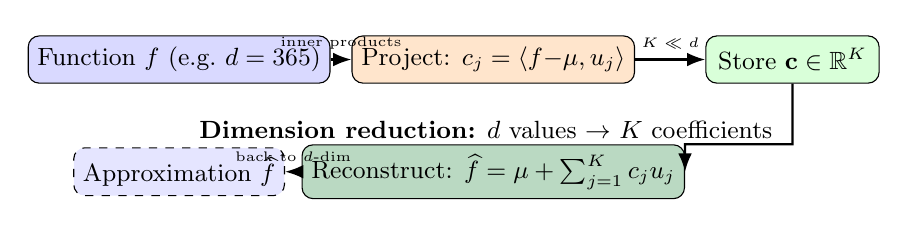
\begin{tikzpicture}[scale=0.95, every node/.style={font=\small}, box/.style={draw, rounded corners, minimum height=0.6cm, minimum width=2.2cm}, arrow/.style={-Latex, thick}]
    \node[box, fill=blue!15] (orig) at (0,0) {Function $f$ (e.g.\ $d=365$)};
    \node[box, fill=orange!20] (proj) at (4.2,0) {Project: $c_j = \langle f{-}\mu, u_j \rangle$};
    \node[box, fill=green!15] (store) at (8.2,0) {Store $\mathbf{c} \in \mathbb{R}^K$};
    \draw[arrow] (orig) -- (proj) node[midway, above, font=\tiny] {inner products};
    \draw[arrow] (proj) -- (store) node[midway, above, font=\tiny] {$K \ll d$};
    \node[below] at (4.1,-0.7) {\textbf{Dimension reduction:} $d$ values $\to$ $K$ coefficients};
    \node[box, fill=recon3color!30] (recon) at (4.2,-1.5) {Reconstruct: $\widehat{f} = \mu + \sum_{j=1}^K c_j u_j$};
    \node[box, fill=blue!10, dashed] (approx) at (0,-1.5) {Approximation $\widehat{f}$};
    \draw[arrow] (store) -- (store |- recon.north) -| (recon.east);
    \draw[arrow] (recon.west) -- (approx.east) node[midway, above, font=\tiny] {back to $d$-dim};
  \end{tikzpicture}
  \end{center}
  \vspace{0.25cm}
  \textbf{Summary:} Keep only $\mathbf{c} = (c_1, \ldots, c_K)$; reconstruct when needed. Compression, comparison, and downstream analysis use $K$-dim vectors instead of $d$-dim.
\end{frame}

% --- Real-world: where do "functions" come from? ---
\begin{frame}{Real-world functions: two examples}
  \small
  \textbf{1. Weather (e.g.\ SNWD — snow depth)}
  \begin{itemize}
    \item One ``function'' = one \textbf{station--year}: snow depth on each of 365 days.
    \item Data matrix: rows = station-years, columns = day-of-year (grid points).
    \item Mean = average seasonal pattern; PCs = main modes of variation (e.g.\ overall depth, early vs late winter).
  \end{itemize}
  \vspace{0.25cm}
  \textbf{2. NYC taxi demand}
  \begin{itemize}
    \item One ``function'' = a \textbf{time series}: e.g.\ pickups per hour over a day (or cabs per minute by source/destination).
    \item Data matrix: rows = days or (source, destination) pairs, columns = time bins.
    \item Mean = average daily pattern; PCs = main modes (e.g.\ rush hours, weekend vs weekday).
  \end{itemize}
  \vspace{0.15cm}
  In both cases: PCA gives a data-driven basis; we approximate and summarize each function by top-$K$ coefficients.
\end{frame}

% --- Weather PCA (SNWD) ---
\begin{frame}{Weather PCA: snow depth (SNWD)}
  \small
  \textbf{Data:} \texttt{weather/PCA\_Analysis/PCA\_reconstruction} (and \texttt{compute\_PCA\_vectors}).
  \begin{itemize}
    \item Each row: one \textbf{station--year}; columns = \texttt{day\_1}, \ldots, \texttt{day\_365} (snow depth).
    \item Center by \textbf{mean vector} $\boldsymbol{\mu}$ (average snow depth per day-of-year).
    \item \textbf{Principal components}: orthonormal vectors of length 365; ordered by explained variance.
    \item \textbf{Reconstruction}: $\widehat{f} = \boldsymbol{\mu} + \sum_{j=1}^K c_j \mathbf{u}_j$; MSE/MAE measure error.
  \end{itemize}
  \vspace{0.2cm}
  \textbf{Summarizing a station--year:} store only $(c_1, \ldots, c_K)$ (top-$K$ PCA coefficients).\\
  Used for: compression, comparison across stations/years, or as features for models.
\end{frame}

\begin{frame}{Weather PCA: actual function and approximation (SNWD)}
  \small
  One station--year: \textbf{original} snow depth (day 1--365) and \textbf{reconstructions} using mean only (1 term), mean + 1 PC (2 terms), mean + 2 PCs (3 terms).
  \vspace{0.2cm}
  \begin{center}
    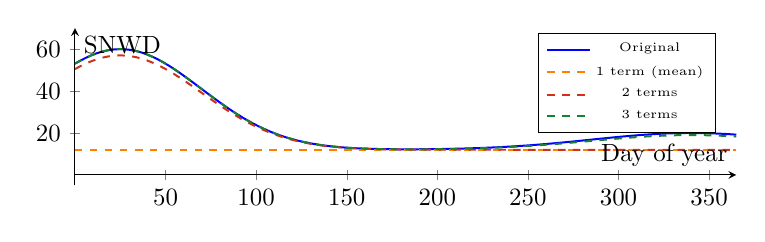
\begin{tikzpicture}[scale=0.9]
      \begin{axis}[
          width=0.9\textwidth, height=3.8cm,
          xmin=0, xmax=365, ymin=-5, ymax=70,
          axis lines=middle,
          xlabel={Day of year}, ylabel={SNWD},
          legend pos=north east,
          legend style={font=\tiny}
        ]
        % Plausible winter peak (snow depth): peak near day 30 (Jan) and shallow secondary
        \addplot[blue, thick, domain=0:365, samples=120] {12 + 48*exp(-(x-25)^2/4000) + 8*exp(-(x-340)^2/6000)};
        \addplot[orange, thick, dashed, domain=0:365, samples=80] {12};
        \addplot[recon2color, thick, dashed, domain=0:365, samples=120] {12 + 45*exp(-(x-25)^2/4000)};
        \addplot[recon3color, thick, dashed, domain=0:365, samples=120] {12 + 48*exp(-(x-25)^2/4000) + 7*exp(-(x-340)^2/6000)};
        \legend{Original, 1 term (mean), 2 terms, 3 terms}
      \end{axis}
    \end{tikzpicture}
  \end{center}
  As $K$ increases, the reconstruction approaches the original; the \textbf{summary} $(c_1,\ldots,c_K)$ captures the curve with few numbers.
\end{frame}

% --- NYC Taxi PCA ---
\begin{frame}{NYC taxi PCA analysis}
  \small
  \textbf{PCA of continuous variables} (fare, distance, duration, etc.): standard multivariate PCA; eigenvectors and eigenvalues describe which linear combinations vary most.
  \vspace{0.2cm}
  \textbf{Functions as time series} (e.g.\ demand over time):
  \begin{itemize}
    \item \textbf{Mean cabs per minute} (or per hour) for different source/destination pairs $\Rightarrow$ one ``mean function'' per pair or one overall mean over time bins.
    \item Each \textbf{function} = one day (or one pair): values in each time bin.
    \item \textbf{Eigenvectors} of the covariance of these time series = principal component \emph{functions} (e.g.\ peak vs off-peak pattern).
    \item \textbf{Coefficients} of the PCA depend on: which day, which source/destination, time of day, etc.; they summarize how much each PC contributes.
  \end{itemize}
  \vspace{0.15cm}
  Same idea: approximate and summarize each curve by top-$K$ coefficients.
\end{frame}

\begin{frame}{NYC taxi: actual function and approximation (demand)}
  \small
  One day (or one source--destination pair): \textbf{original} demand (e.g.\ pickups per hour, 0--24) and \textbf{reconstructions} with 1 term (mean), 2 terms, 3 terms.
  \vspace{0.2cm}
  \begin{center}
    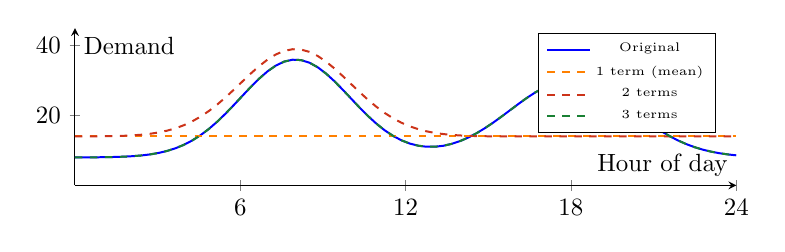
\begin{tikzpicture}[scale=0.9]
      \begin{axis}[
          width=0.9\textwidth, height=3.8cm,
          xmin=0, xmax=24, ymin=0, ymax=45,
          axis lines=middle,
          xlabel={Hour of day}, ylabel={Demand},
          legend pos=north east,
          legend style={font=\tiny},
          xtick={0,6,12,18,24}
        ]
        % Two peaks: morning ~8, evening ~18
        \addplot[blue, thick, domain=0:24, samples=80] {8 + 28*exp(-(x-8)^2/8) + 22*exp(-(x-18)^2/10)};
        \addplot[orange, thick, dashed, domain=0:24, samples=40] {14};
        \addplot[recon2color, thick, dashed, domain=0:24, samples=80] {14 + 25*exp(-(x-8)^2/8)};
        \addplot[recon3color, thick, dashed, domain=0:24, samples=80] {8 + 28*exp(-(x-8)^2/8) + 22*exp(-(x-18)^2/10)};
        \legend{Original, 1 term (mean), 2 terms, 3 terms}
      \end{axis}
    \end{tikzpicture}
  \end{center}
  Mean captures average level; first PC often aligns with morning rush; adding PCs refines evening peak and shape. \textbf{Summary} $(c_1,\ldots,c_K)$ describes the day's pattern compactly.
\end{frame}

% --- Figure: target and reconstructions (like notebook last slide) ---
\begin{frame}{Example: $f(x) = |x-2|$ on $[0, 2\pi]$}
  \small
  Orthonormal basis $\{1, \cos x, \sin x\}$ (or first 3 PCs of a suitable dataset).\\
  Reconstruction with 1, 2, or 3 terms (same idea as \texttt{Functions\_as\_vectors}).
  \vspace{0.15cm}
  \begin{center}
    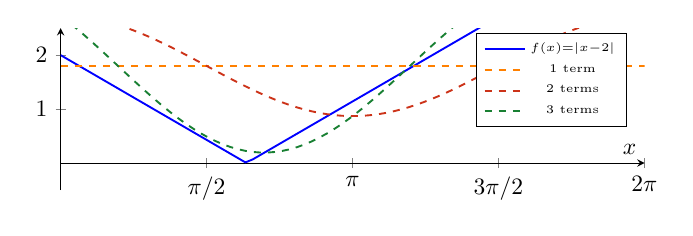
\begin{tikzpicture}[scale=0.85]
      \begin{axis}[
          width=0.85\textwidth, height=4cm,
          xmin=0, xmax=2*pi, ymin=-0.5, ymax=2.5,
          axis lines=middle,
          xlabel={$x$}, ylabel={},
          xtick={0, 1.57, 3.14, 4.71, 6.28},
          xticklabels={0, $\pi/2$, $\pi$, $3\pi/2$, $2\pi$},
          legend pos=north east,
          legend style={font=\tiny}
        ]
        \addplot[blue, thick, domain=0:2*pi, samples=80] {abs(x-2)};
        \addplot[orange, thick, dashed, domain=0:2*pi, samples=80] {1.8};
        \addplot[recon2color, thick, dashed, domain=0:2*pi, samples=80] {1.8 + 0.93*cos(deg(x))};
        \addplot[recon3color, thick, dashed, domain=0:2*pi, samples=80] {1.8 + 0.93*cos(deg(x)) - 1.31*sin(deg(x))};
        \legend{$f(x){=}|x{-}2|$, 1 term, 2 terms, 3 terms}
      \end{axis}
    \end{tikzpicture}
  \end{center}
  \textbf{Summary} with $K=3$: $\mathbf{c} \approx (1.8,\, 0.93,\, -1.31)$ (coefficients of constant, $\cos$, $\sin$).
\end{frame}

% --- Optional: mean and PC functions ---
\begin{frame}{Mean and principal component functions (sketch)}
  \small
  Same setting: basis $\{1, \cos x, \sin x\}$ on $[0, 2\pi]$. ``Mean'' and ``PCs'' can be chosen to match the previous slide.
  \vspace{0.15cm}
  \begin{center}
    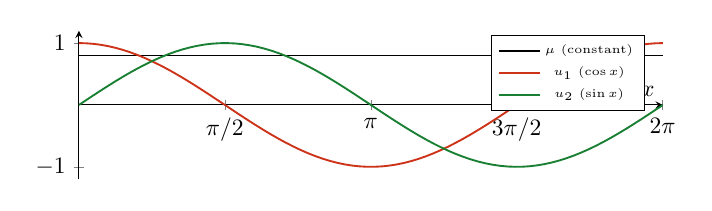
\begin{tikzpicture}[scale=0.85]
      \begin{axis}[
          width=0.85\textwidth, height=3.8cm,
          xmin=0, xmax=2*pi, ymin=-1.2, ymax=1.2,
          axis lines=middle,
          xlabel={$x$}, ylabel={},
          xtick={0, 1.57, 3.14, 4.71, 6.28},
          xticklabels={0, $\pi/2$, $\pi$, $3\pi/2$, $2\pi$},
          legend pos=north east,
          legend style={font=\tiny}
        ]
        \addplot[black, thick, domain=0:2*pi, samples=80] {0.8};
        \addplot[recon2color, thick, domain=0:2*pi, samples=80] {cos(deg(x))};
        \addplot[recon3color, thick, domain=0:2*pi, samples=80] {sin(deg(x))};
        \legend{$\mu$ (constant), $u_1$ ($\cos x$), $u_2$ ($\sin x$)}
      \end{axis}
    \end{tikzpicture}
  \end{center}
  Approximating $f$: $f \approx \mu + c_1 u_1 + c_2 u_2 + \cdots$.
\end{frame}

% --- Recap ---
\begin{frame}{Recap}
  \small
  \begin{itemize}
    \item \textbf{Functions as vectors} on a grid; PCA uses a data-driven orthonormal basis (PCs).
    \item \textbf{Data:} matrix of $n$ functions (rows), centered by the mean function $\mu$.
    \item \textbf{Principal component functions} $u_1, u_2, \ldots$: orthonormal, variance-ordered.
    \item \textbf{Approximation:} $f \approx \mu + \sum_{j=1}^K c_j u_j$ with $c_j = \langle f - \mu, u_j \rangle$.
    \item \textbf{Summary} of $f$: coefficient vector $\mathbf{c} = (c_1, \ldots, c_K)$ for the top $K$ PCs.
    \item \textbf{Real-world:} Weather (SNWD) = station--year $\times$ day-of-year; NYC taxi = demand time series or PCA of continuous variables; both use the same approximation and summary workflow.
  \end{itemize}
\end{frame}

\end{document}
